\documentclass[a4paper,11pt,twoside]{memoir}
\chapterstyle{veelo}

\usepackage{TUINFDA}

\usepackage{url}
\usepackage{hyperref}					% links in pdf
\usepackage{graphicx}            			% Figures
\usepackage{verbatim}            			% Code-Environment
\usepackage[lined,linesnumbered,algochapter]{algorithm2e} % Algorithm-Environment

\usepackage{pgf}					
\usepackage{tikz}					% tikz graphics
\usetikzlibrary{arrows,automata}

\usepackage{ngerman}
\usepackage[ngerman]{babel}
\usepackage{bibgerm,cite}       % Deutsche Bezeichnungen, Automatisches Zusammenfassen von Literaturstellen
\usepackage[ngerman]{varioref}  % Querverweise
% to use the german charset include cp850 for MS-DOS, ansinew for Windows and latin1 for Linux.
% \usepackage[latin1]{inputenc}

\thesistitle{Title of the Thesis}
\thesissubtitle{Optional Subtitle} % optional
\thesisdate{TT.MM.JJJJ}

% all titles and designations have to be gender-related!
\thesisdegree{Diplom-Ingenieurin}{Diplom-Ingenieurin}
\thesiscurriculum{Wirtschaftsinformatik}{Business Informatics} % your study
\thesisverfassung{Verfasserin} % Verfasser
\thesisauthor{Martina Musterfrau} % your name
\thesisauthoraddress{Musterplatz 1, 1111 Wien} % your address
\thesismatrikelno{0123456} % your registration number

\thesisbetreins{o.Univ.-Prof. Dipl.-Ing. Mag. Dr. Monika Musterprofessorin}
\thesisbetrzwei{Dr. Vorname Familienname}
\thesisbetrdrei{Dr. Vorname Familienname} % optional

% define page numbering styles
\makepagestyle{numberCorner}
\makeevenfoot{numberCorner}{\thepage}{}{}
\makeoddfoot{numberCorner}{}{}{\thepage}

% define custom macros for specific formats or names
\newcommand{\uml}[1]{\texttt{#1}}
\newcommand{\cd}{\textsf{Class Diagram}}

\begin{document}

\captionnamefont{\bfseries}

%%%%%%%%%%%%%%%%%%%%%%%%%%%%%%%%%%%%%%%%%
%%%   FRONTMATTER    %%%%%%%%%%%%%%%%%%%%
%%%%%%%%%%%%%%%%%%%%%%%%%%%%%%%%%%%%%%%%%
\frontmatter
\pagenumbering{roman}

%%%%%%%%%%%%%%%%%%%%%%%%%%%%%%%%%%%%%%%%%
%%%   TITLEPAGES    %%%%%%%%%%%%%%%%%%%%%
%%%%%%%%%%%%%%%%%%%%%%%%%%%%%%%%%%%%%%%%%

% the german title page is required as first page
% $Id: titlepage.tex 1752 2010-03-20 11:07:02Z tkren $
%
% TU Wien - Faculty of Informatics
% thesis titlepage
%
% This titlepage is using the geometry package, see
% <http://www.ctan.org/macros/latex/contrib/geometry/geometry.pdf>
%
% For questions and comments send an email to
% Thomas Krennwallner <tkren@kr.tuwien.ac.at>
% or to Petra Brosch <brosch@big.tuwien.ac.at>
%

\selectlanguage{ngerman}

% setup page dimensions for titlepage
\newgeometry{left=2.4cm,right=2.4cm,bottom=2.5cm,top=2cm}

% force baselineskip and parindent
\newlength{\tmpbaselineskip}
\setlength{\tmpbaselineskip}{\baselineskip}
\setlength{\baselineskip}{13.6pt}
\newlength{\tmpparindent}
\setlength{\tmpparindent}{\parindent}
\setlength{\parindent}{17pt}

% first titlepage
\thispagestyle{tuinftitlepage}

%
% Kludge: for each titlepage set \pagenumbering to a different
% style. This is used to fix a problem with hyperref, because there
% are multiple "page 1" and hyperref hates that
%
\pagenumbering{Alph}

\begin{center}
{\ \vspace{3.4cm}}

\begin{minipage}[t][2.8cm][s]{\textwidth}%
\centering
\thesistitlefontHUGE\sffamily\bfseries\tuinfthesistitle\\
\bigskip
{\thesistitlefonthuge\sffamily\bfseries\tuinfthesissubtitle}
\end{minipage}

\vspace{1.3cm}

{\thesistitlefontLARGE\sffamily \tuinfthesistype}

\vspace{6mm}

{\thesistitlefontlarge\sffamily zur Erlangung des akademischen Grades}

\vspace{6mm}

{\thesistitlefontLARGE\sffamily\bfseries \tuinfthesisdegree}

\vspace{6mm}

{\thesistitlefontlarge\sffamily im Rahmen des Studiums}

\vspace{6mm}

{\thesistitlefontLarge\sffamily\bfseries \tuinfthesiscurriculum}

\vspace{6.5mm}

{\thesistitlefontlarge\sffamily eingereicht von}

\vspace{6mm}

{\thesistitlefontLarge\sffamily\bfseries \tuinfthesisauthor}

\vspace{1.5mm}

{\thesistitlefontlarge\sffamily Matrikelnummer \tuinfthesismatrikelno} 

\vspace{1.4cm}

\vspace{0pt}\raggedright\thesistitlefontnormalsize\sffamily
\begin{minipage}[t][1.6cm][t]{\textwidth}%
  %
  an der

  Fakult\"{a}t f\"{u}r Informatik der Technischen Universit\"{a}t Wien
\end{minipage}

\begin{minipage}[t][4cm][t]{\textwidth}%
  \vspace{0pt}\raggedright\thesistitlefontnormalsize\sffamily
  %
  \begin{tabbing}%
	    \hspace{19mm} \= \hspace{66mm} \kill
	    \tuinfthesisbetreuung: \> \tuinfthesisbetreins\\
	    Mitwirkung: \> \tuinfthesisbetrzwei\\
	                \> \tuinfthesisbetrdrei
  \end{tabbing}
\end{minipage}

\begin{minipage}[t][1.5cm][t]{\textwidth}%
  \vspace{0pt}\sffamily\thesistitlefontnormalsize
  \begin{tabbing}%
    \hspace{45mm} \= \hspace{63mm} \= \hspace{51mm} \kill
    Wien, \tuinfthesisdate \> {\raggedright\rule{51mm}{0.5pt}} \> {\raggedright\rule{51mm}{0.5pt}} \\
    \> \begin{minipage}[t][0.5cm][t]{51mm}\centering (Unterschrift \tuinfthesisverfassung)\end{minipage}
    \> \begin{minipage}[t][0.5cm][t]{51mm}\centering (Unterschrift \tuinfthesisbetreuung)\end{minipage}
    \end{tabbing}
\end{minipage}

\end{center}

% we want an empty page right after first titlepage
\pagestyle{empty}
\cleardoublepage

% we're done with the titlepages, proceed with default pagenumbering
\pagenumbering{roman}

% restore baselineskip
\setlength{\baselineskip}{\tmpbaselineskip}
\setlength{\parindent}{\tmpparindent}

% back to normal geometry
\restoregeometry

\selectlanguage{english}

%%% Local Variables:
%%% TeX-PDF-mode: t
%%% TeX-debug-bad-boxes: t
%%% TeX-parse-self: t
%%% TeX-auto-save: t
%%% reftex-plug-into-AUCTeX: t
%%% End:


% an english translation may follow
% $Id: titlepage.tex 1752 2010-03-20 11:07:02Z tkren $
%
% TU Wien - Faculty of Informatics
% thesis titlepage
%
% This titlepage is using the geometry package, see
% <http://www.ctan.org/macros/latex/contrib/geometry/geometry.pdf>
%
% For questions and comments send an email to
% Thomas Krennwallner <tkren@kr.tuwien.ac.at>
% or to Petra Brosch <brosch@big.tuwien.ac.at>
%

% setup page dimensions for titlepage
\newgeometry{left=2.4cm,right=2.4cm,bottom=2.5cm,top=2cm}

% force baselineskip and parindent
%\newlength{\tmpbaselineskip}
%\setlength{\tmpbaselineskip}{\baselineskip}
%\setlength{\baselineskip}{13.6pt}
%\newlength{\tmpparindent}
%\setlength{\tmpparindent}{\parindent}
%\setlength{\parindent}{17pt}

% first titlepage
\thispagestyle{tuinftitlepage}

%
% Kludge: for each titlepage set \pagenumbering to a different
% style. This is used to fix a problem with hyperref, because there
% are multiple "page 1" and hyperref hates that
%
\pagenumbering{Roman}

\begin{center}
{\ \vspace{3.4cm}}

\begin{minipage}[t][2.8cm][s]{\textwidth}%
\centering
\thesistitlefontHUGE\sffamily\bfseries\tuinfthesistitle\\
\bigskip
{\thesistitlefonthuge\sffamily\bfseries\tuinfthesissubtitle}
\end{minipage}

\vspace{1.3cm}

{\thesistitlefontLARGE\sffamily \tuinfthesistypeen}

\vspace{6mm}

{\thesistitlefontlarge\sffamily submitted in partial fulfillment of the requirements for the degree of}

\vspace{6mm}

{\thesistitlefontLARGE\sffamily\bfseries \tuinfthesisdegreeen}

\vspace{6mm}

{\thesistitlefontlarge\sffamily in}

\vspace{6mm}

{\thesistitlefontLarge\sffamily\bfseries \tuinfthesiscurriculumen}

\vspace{6.5mm}

{\thesistitlefontlarge\sffamily by}

\vspace{6mm}

{\thesistitlefontLarge\sffamily\bfseries \tuinfthesisauthor}

\vspace{1.5mm}

{\thesistitlefontlarge\sffamily Registration Number \tuinfthesismatrikelno} 

\vspace{1.4cm}

\begin{minipage}[t][1.6cm][t]{\textwidth}%
  \vspace{0pt}\raggedright\thesistitlefontnormalsize\sffamily
  %
  to the Faculty of Informatics 

  at the Vienna University of Technology
\end{minipage}

\vspace{0pt}\raggedright\thesistitlefontnormalsize\sffamily
\begin{minipage}[t][4cm][t]{\textwidth}%
  \begin{tabbing}%
	    \hspace{19mm} \= \hspace{66mm} \kill
	    Advisor: \> \tuinfthesisbetreins\\
%	    Assistance: \> \tuinfthesisbetrzwei\\
%	                \> \tuinfthesisbetrdrei
     \end{tabbing}
\end{minipage}

\begin{minipage}[t][1.5cm][t]{\textwidth}%
  \vspace{0pt}\sffamily\thesistitlefontnormalsize
  \begin{tabbing}%
    \hspace{45mm} \= \hspace{63mm} \= \hspace{51mm} \kill
    Vienna, \tuinfthesisdate \> {\raggedright\rule{51mm}{0.5pt}} \> {\raggedright\rule{51mm}{0.5pt}} \\
    \> \begin{minipage}[t][0.5cm][t]{51mm}\centering (Signature of Author)\end{minipage}
    \> \begin{minipage}[t][0.5cm][t]{51mm}\centering (Signature of Advisor)\end{minipage}
    \end{tabbing}
\end{minipage}

\end{center}

% we want an empty page right after first titlepage
\pagestyle{empty}
\cleardoublepage

% we're done with the titlepages, proceed with default pagenumbering
\pagenumbering{roman}

% restore baselineskip
\setlength{\baselineskip}{\tmpbaselineskip}
\setlength{\parindent}{\tmpparindent}

% back to normal geometry
\restoregeometry


%%% Local Variables:
%%% TeX-PDF-mode: t
%%% TeX-debug-bad-boxes: t
%%% TeX-parse-self: t
%%% TeX-auto-save: t
%%% reftex-plug-into-AUCTeX: t
%%% End:
 % optional

%%%%%%%%%%%%%%%%%%%%%%%%%%%%%%%%%%%%%%%%%
%%%   ERKLAERUNG DER SELBSTAENDIGKEIT   %
%%%%%%%%%%%%%%%%%%%%%%%%%%%%%%%%%%%%%%%%%
\cleardoublepage
\selectlanguage{ngerman}
\chapter*{Erklärung zur Verfassung der Arbeit}

\tuinfthesisauthor\\
\tuinfthesisauthoraddress

\vspace*{1.2cm}

Hiermit erkläre ich, dass ich diese Arbeit selbständig verfasst habe, 
dass ich die verwendeten Quellen und Hilfsmittel vollständig angegeben 
habe und dass ich die Stellen der Arbeit - einschließlich Tabellen, 
Karten und Abbildungen -, die anderen Werken oder dem Internet im 
Wortlaut oder dem Sinn nach entnommen sind, auf jeden Fall unter Angabe 
der Quelle als Entlehnung kenntlich gemacht habe.\\

\vspace*{2cm}
\begin{tabbing}%
    \hspace{58mm} \= \hspace{28mm} \= \hspace{58mm} \kill
    {\raggedright\rule{58mm}{0.5pt}} \> \> {\raggedright\rule{58mm}{0.5pt}} \\
    \begin{minipage}[t][0.5cm][t]{58mm}
	\vspace{0pt}\sffamily\thesistitlefontnormalsize
	\centering (Ort, Datum)
    \end{minipage}
    \> \>
    \begin{minipage}[t][0.5cm][t]{58mm}
	\vspace{0pt}\sffamily\thesistitlefontnormalsize
	\centering (Unterschrift \tuinfthesisverfassung)
    \end{minipage}
\end{tabbing}


\selectlanguage{english}

%%%%%%%%%%%%%%%%%%%%%%%%%%%%%%%%%%%%%%%%%
%%%   ACKNOWLEDGEMENTS    %%%%%%%%%%%%%%%
%%%%%%%%%%%%%%%%%%%%%%%%%%%%%%%%%%%%%%%%%

% optional acknowledgements may be included in german or in english
%\chapter*{Danksagung}

Hier fügen Sie optional eine Danksagung ein.
 		% optional
\chapter*{Acknowledgements}

Optional acknowledgements may be inserted here.	% optional

%%%%%%%%%%%%%%%%%%%%%%%%%%%%%%%%%%%%%%%%%
%%%   ABSTARCT    %%%%%%%%%%%%%%%%%%%%%%%
%%%%%%%%%%%%%%%%%%%%%%%%%%%%%%%%%%%%%%%%%

\chapter*{Abstract}

According to the guidelines of the faculty, an abstract in English has to be inserted here.
\cleardoublepage
\selectlanguage{ngerman}
\chapter*{Kurzfassung}

% Since the dawn of computer graphics natural phenomena have served as a permanent topic of interest for researchers and enthusiasts.
% To reproduce nature's elegance and beauty has proven to be a task of immense complexity. Skylight, clouds, a sunset. Water in various environments.
% Glass of water generating caustics. A child exploring fluid dynamics in the bathtub. A lake at rest, reflecting the surrounding mountains.
% The endless ocean bearing detail on every scale: the foam and spray caused by breaking waves, the glimmer on the ocean surface caused by waves
% with wavelengths smaller than a centimeter, the subtle shift in water color depending on the local underwater flora and fauna.

Die realistische Darstellung von Wasseroberflächen ist seit jeher ein beliebtes Forschungsthema in der Computergraphik, und vor allem in
der Echtzeitgraphik. Den weiten Ozean in Echtzeit darzustellen ist
eine besondere Herausforderung. Die Gründe hierfür sind vielseitig.
%Unter anderem ist der Ozean ein riesiges Gewässer, und dem Beobachter
%ist es möglich rasch zwischen einer Nahaufnahme und einem Panorama
%zu wechseln.
Unter anderem ist der Ozean ein riesiges Gewässer, welches wir auf
sehr unterschiedliche Art und Weise abbilden möchten, von der Nahaufnahme
bis zum weitläufigen Panorama.
Weiters ist der Ozean ein sehr komplexes, dynamisches System das aus
einer riesigen Anzahl Wellen unterschiedlicher Größen besteht, vom
riesigen Tsunami bis zu millimeterkleinen Kapillarwellen.

Wir präsentieren in dieser Arbeit Algorithmen um den weiten Ozean
nicht nur in Echtzeit zu rendern, sondern auch alle dafür benötigten
Daten in Echtzeit zu generieren. Unser Fokus liegt darauf, glaubhafte
Ozeanoberflächen mittels Wellenspektren zu erzeugen, wobei letztere dem Forschungsbereich der Ozeanographie entspringen.
Wir untersuchen unterschiedliche Wellenspektren sowohl auf ihre
Eigenheiten, als auch auf ihre Eignung für die Darstellung mittels Echtzeitgraphik-Algorithmen. Zusätzlich erläutern wir
die notwendigen Hintergründe um unterschiedlich Wellenspektren sinnvoll
in eine gemeinsames Grundstruktur zu integrieren. Selbige erlaubt es uns
schlussendlich, unabhängig vom gewählten Wellenspektrum, nicht nur glaubhafte, sondern auch stimmige Ozeanoberflächen zu erzeugen.
 
%
%The synthesis of a believable depiction of the ocean surface is a permanent
%topic of interest in computer graphics. It represents even more of a
%challenge for applications which require the real-time display of a water
%body as large as the ocean.
%That is because the ocean is a highly dynamic system which combines waves
%at all scales, ranging from millimetres to kilometres. Moreover, the
%ocean may be observed from several distances, ranging from close-ups
%to views which reach the horizon. 
%%To complicate matters further, the
%%ocean is illuminated by natural light sources, such as the sun and the
%%sky, which are dynamic by nature too.
%Thus, we present a framework to generate and render the open ocean in
%real time, for arbitrary viewing distances and including waves at all
%scales. We focus our efforts on the geometry of the animated
%ocean surface, for which we leverage a set of wave spectrum models from
%oceanographic research. We discuss the intricacies of
%said models, as well as their fitness for real-time rendering. Moreover,
%we delineate in detail how to integrate distinct wave spectrum models into a
%coherent framework, from which one is able obtain believable, consistent
%and coherent results.

%The scope of this thesis includes the generation, animation and rendering of the
%surface of an open ocean in real-time. We focus our interest on the synthesis of
%animated ocean surface geometry, for which we will adopt a set of models from
%oceanographic research. Specific properties of said models allow for
%easy addition and reduction of detail, as well as for a range of algorithmic
%optimizations. The former combined with the latter gives us the opportunity to
%strike a well-adjusted balance between model detail and computational workload,
%and thereby to improve upon the status quo of current implementations.

%Realistic animation and rendering of the ocean is an important aspect for simulators, movies and video games.
%By nature, the ocean is a difficult problem for Computer Graphics: it is a dynamic system, it combines wave trains
%at all scales, ranging from kilometric to millimetric. Worse, the ocean is usually viewed at several distances, from
%very close to the viewpoint to the horizon, increasing the multi-scale issue, and resulting in aliasing problems. The
%illumination comes from natural light sources (the Sun and the sky dome), is also dynamic, and often underlines
%the aliasing issues. In this paper, we present a new algorithm for modelling, animation, illumination and rendering
%of the ocean, in real-time, at all scales and for all viewing distances. Our algorithm is based on a hierarchical
%representation, combining geometry, normals and BRDF. For each viewing distance, we compute a simplified
%version of the geometry, and encode the missing details into the normal and the BRDF, depending on the level of
%detail required. We then use this hierarchical representation for illumination and rendering. Our algorithm runs
%in real-time, and produces highly realistic pictures and animations.

%Natural phenomena are a permanent topic of interest for computer graphics researchers and enthusiasts. To synthesise a believable
%depiction of an ocean surface is a complex task, especially in realtime rendering. The first part of our work will discuss the
%challenges posed by the task at hand, and discuss a variety of current approaches to the problem. The second part will present
%our give an
%overview of the underlying wave theory as well as the different oceanographic models employed in this work.
\selectlanguage{english}

%%%%%%%%%%%%%%%%%%%%%%%%%%%%%%%%%%%%%%%%%
%%%   CONTENTS    %%%%%%%%%%%%%%%%%%%%%%%
%%%%%%%%%%%%%%%%%%%%%%%%%%%%%%%%%%%%%%%%%
% uncomment to set document language to german (results in "Inhaltsverzeichnis", "Kapitel", "Abbildung", etc. instead of "Contents", "Chapter", and "Figure"), otherwise the document's language is english
%\selectlanguage{ngerman}

\setcounter{tocdepth}{1}

\cleardoublepage
\pagestyle{numberCorner}
\tableofcontents*

%%%%%%%%%%%%%%%%%%%%%%%%%%%%%%%%%%%%%%%%%
%%%   MAINMATTER    %%%%%%%%%%%%%%%%%%%%%
%%%%%%%%%%%%%%%%%%%%%%%%%%%%%%%%%%%%%%%%%

\mainmatter
\pagenumbering{arabic}
\pagestyle{numberCorner}

%%%%%%%%%%%%%%%%%%%%%%%%%%%%%%%%%%%%%%%%%
\chapter{Introduction}
\label{ch:intro}
%%%%%%%%%%%%%%%%%%%%%%%%%%%%%%%%%%%%%%%%%

\chapter{Introduction}
\label{ch:intro}
%
Natural phenomena are a challenging topic in the field of computer graphics.
Actual examples are complex structures which are to be found throughout nature,
such as mountains, trees and water. The latter is especially interesting
because of its highly dynamic form which poses a variety of sophisticated problems.
%
\section{Motivation}
\label{sec:motivation}
For computer graphics to reproduce the diverse appearance of ocean surfaces
represents one such problem. But to cover all the dynamics as well
as the lighting of an entire ocean would exceed the scope of this work.
We may approach a more specific subject, namely the synthesis of animated ocean
surfaces which are both believable and computationally feasible.
Fortunately, the oceanographic research community did already develop models
which satisfy those requirements, as they are essential for oceanographic
simulations. Therefore, we combine consolidated findings from oceanographic
research with computer graphics algorithms to complete the task at hand.
%
% believable ocean surface geometry~\emph{based on} consolidated findings from the
% oceanographic research community.
%
% . We focus our interest on the generation of believable
% ocean surface geometry based on consolidated findings from the oceanographic
% research community.
%
% Based on consolidated findings from the
% oceanographic research community we focus ourselves on the generation of
% believable ocean surface geometry
%
% Hence, our interest focuses on the
% geometry of ocean surfaces using consolidated findings from the oceanographic
% research community.
% 
% In the context of this work we focus our interest on the ocean surfaces.
% 
% In the context of this work we focus our interest on the ever-changing shape of
% ocean surfaces.
% 
% Our interest focuses on the geometry of ocean surfaces using
% consolidated findings from the oceanographic research community.
%
\begin{figure}[h]
\centering
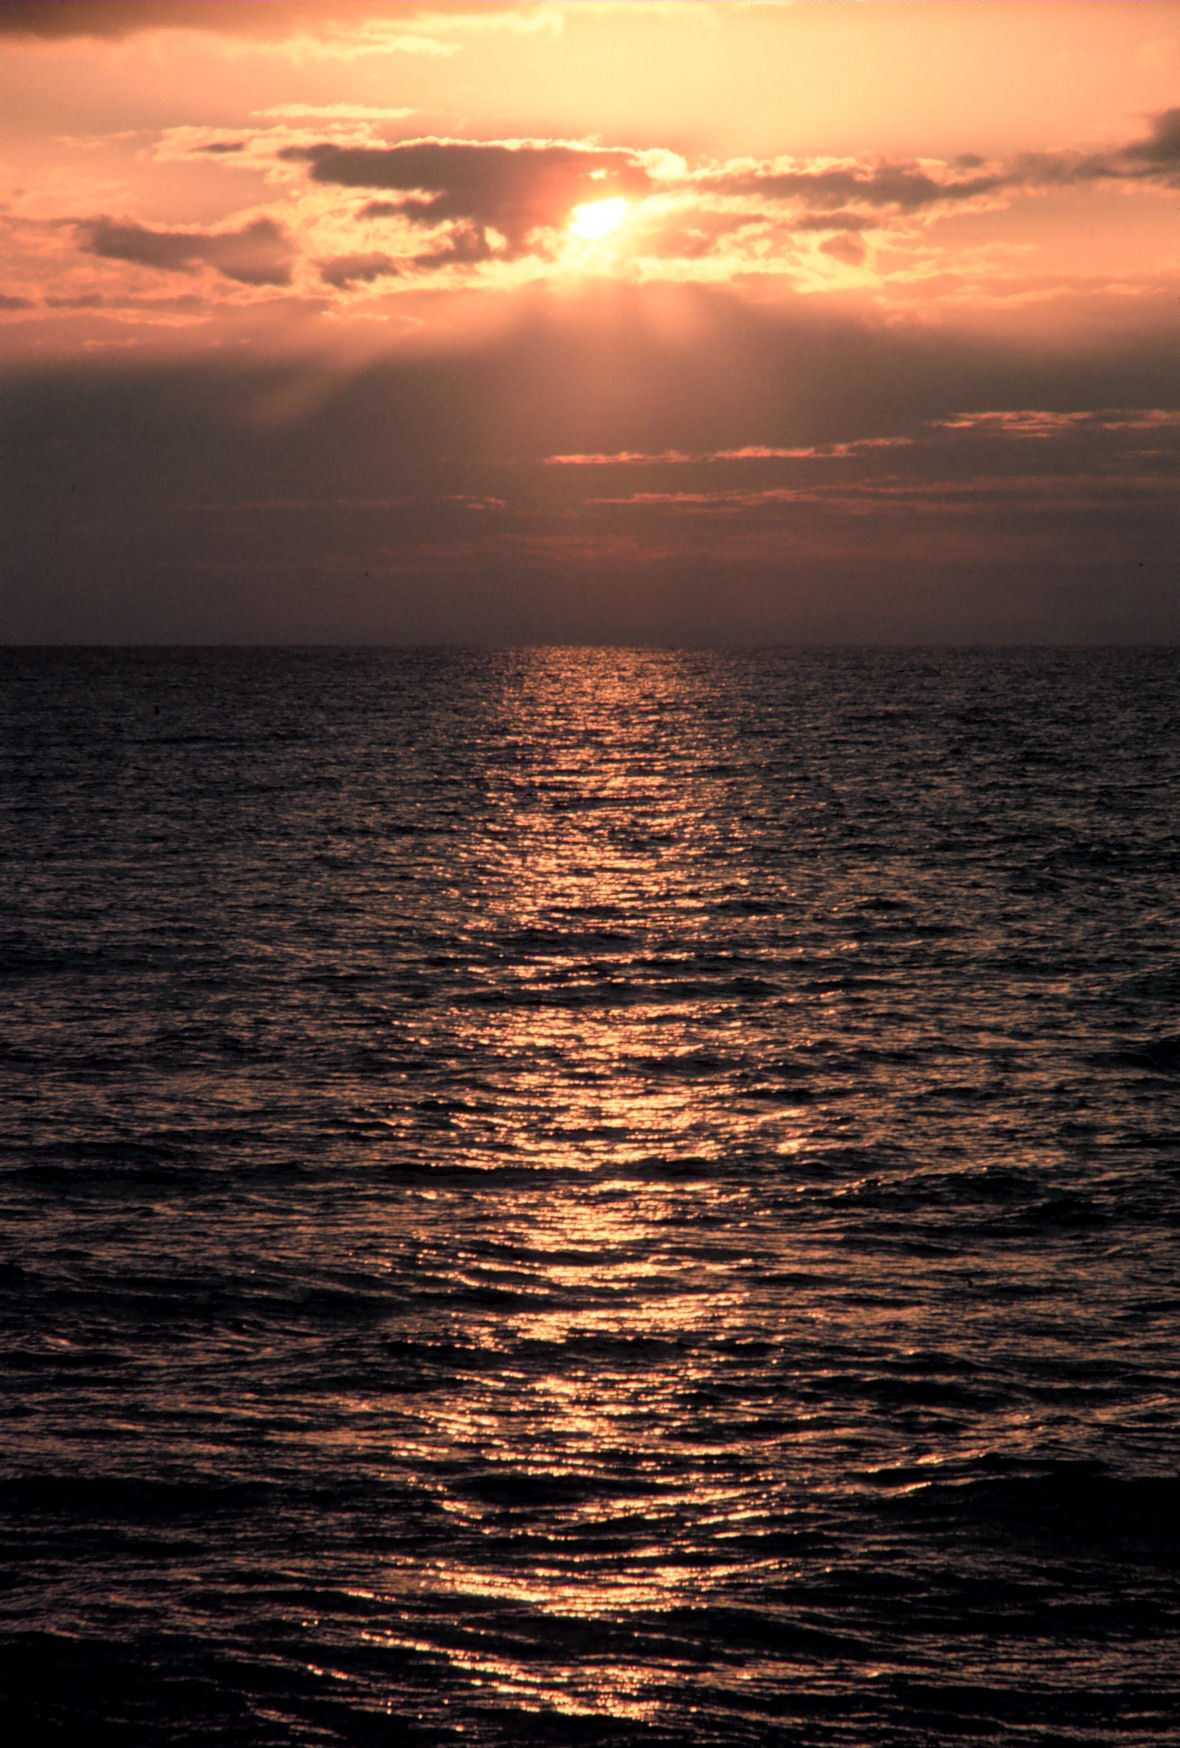
\includegraphics[scale=0.75]{figures/ocean300.jpg}
\caption{The late afternoon sun illuminating the ocean surface. Source: NOAA~\cite{misc:noaa}}
\end{figure}
%
\section{Problem Statement}
\label{sec:problem_statement}
%
Rendering an ocean is a demanding task for several reasons. First, consider the
sheer size of a water body as large as an ocean, which in numerous viewing
situations will be visible all the way to the horizon. Second, the ocean surface
is dynamic, therefore it needs to be constantly updated with the passage of time.
The wave interactions that give the ocean surface its shape are huge in terms of
complexity, thus we employ approximative models published by the oceanographic
research community.
Third, the optics of water are intricate. Incoming light may be reflected at the
surface or may be refracted into the water body, where the ratio between both is
dependent on the angle of incidence between the incoming light and the surface
normal at the point of incidence. Some of the refracted light may find its way
back to the ocean's surface, either by scattering inside the water body or by
reflection at the sea bottom, or possibly by a combination of both. Moreover,
waves on the ocean surface may break and cause surf and foam, both of which
interact with light drastically different than the surrounding water surface.
%
%  adding another
% layer of detail to the visual appearance of the ocean surface.
%
% The visual appearance of an ocean
% surface is highly dependent on its surroundings, because it reflects light from various
% sources e.g the sun, the skydome, clouds, as well as objects close to the
% water surface, such as boats and ships. Water does not only reflect light, it
% also refracts light, where the amount of refracted light to find its way back
% to the water surface is highly dependent on the depth of the water body.
% Moreover, the particulets contained inside the water body interact with the
% refracted light and therefore may cause a tint of the ocean surface.
% In addition, waves may break and cause surf and foam. Both interact with light
% drastically different than the surrounding water surface, adding another layer
% of detail.
%
%
%  (reflections), the depth of the underlying
% water body (refractions), as well as on the particulets contained in the water
% body itself (scattering).
% 
% The generation and animation of a water surface as large as an ocean is a demanding
% task. In most situations will often span all the way to the horizon, 
% 
% Some light is reflected, some is
% refracted, where the latter may or may not find its way back to the water
% surface.
%
\section{Scope and Focus of the Work}
\label{sec:scope_and_focus}
The scope of this thesis includes the generation, animation and rendering of the
surface of an open ocean in real-time. We focus our interest on the synthesis of
animated ocean surface geometry, for which we will adopt a set of mathematical
models from oceanographic research. Specific properties of said models allow for
easy addition and reduction of detail, as well as for a range of algorithmic
optimisations. The former combined with the latter gives us the opportunity to
strike a well-adjusted balance between model detail and computational workload,
and thereby to improve upon the status quo of current implementations.
%
% Note: The oceanographic models discussed in this work are not based on fluid
% dynamics, hence, convincing interaction between the ocean surface and other
% objects is beyond the scope of this thesis.
%
\section{Structure of the Work}
\label{sec:structure}
The remainder of this work is organized as follows: Chapter
\ref{ch:state_of_the_art} gives a survey of ocean simulation and rendering
methods. Chapter~\ref{ch:background} elaborates on the theoretical background
the oceanographic models are based on, as well as on the models themselves.
Chapter~\ref{ch:implementation} describes in detail the
synthesis of all data related to the ocean surface, including both the algorithmic
optimisations and the level of detail mechanism. Furthermore, we give an overview
of the rendering algorithms adopted for our implementation. In Chapter
\ref{ch:summary} we summarize our work and discuss the improvements we were able
to achieve in comparison to the state of the art. Moreover, we will suggest
future work based on open issues of our implementation.


%%%%%%%%%%%%%%%%%%%%%%%%%%%%%%%%%%%%%%%%%
\chapter{Typographic Design}
\label{ch:typo}
%%%%%%%%%%%%%%%%%%%%%%%%%%%%%%%%%%%%%%%%%


For working with LaTeX you can take advantage of a variety of books and free introductions and tutorials on the internet. A competent contact point for LaTeX beginners is the LaTeX Wikibook, which is available under \url{http://en.wikibooks.org/wiki/LaTeX}. 

The following sections give examples of the most important LaTeX environments and commands.

\section{Tables}

Tables have to be realized with the help of the \textit{table} environment. Tables shall be sequentially numbered for each chapter and described in terms of a short caption (cf. Table~\ref{tab:diplomaseminar}).

\begin{table}[htb]
	\centering
	\begin{tabular}{|l|c|c|}
		\hline \textbf{Name} & \textbf{Date} & \textbf{Title} \\
		\hline
		\hline Mustermann Adam  & 18.5   & T1    \\
		\hline Musterfrau Eva  & 22.6   & T2    \\
		\hline
	\end{tabular}
	\caption{Seminar for Master Students}
	\label{tab:diplomaseminar}
\end{table}


\section{Figures}

Like tables, figures shall be sequentially numbered for each chapter and described in terms of a short caption). You could either produce your drawings directly inside Latex using PSTricks\footnote{\url{http://tug.org/PSTricks}}, Tikz\footnote{\url{http://sourceforge.net/projects/pgf}}, or any set of macros dedicated to your requirements (cf. Figure~\ref{fig:samplefigure_tikz}). Alternatively, you may include figures prepared in external tools (cf. Figure~\ref{fig:samplefigure_pdf}). Note, to ensure high quality printing, all figures must have at least 300 dpi.

\begin{figure}
	\centering
	\begin{tikzpicture}[->, auto, node distance=2.8cm, semithick]
	  \node[initial, state] (1)		 {$S_1$};
	  \node[state] 		(2) [right of=1] {$S_2$};
	
	  \path (1) edge [bend left]  node {0} (2)
		(1) edge [loop above] node {1} (1)
		(2) edge [bend left]  node {0} (1)
		(2) edge [loop above] node {1} (2);
	\end{tikzpicture}
	\caption{Sample figure}
	\label{fig:samplefigure_tikz}
\end{figure}

\begin{figure}[tb]
	\centering
	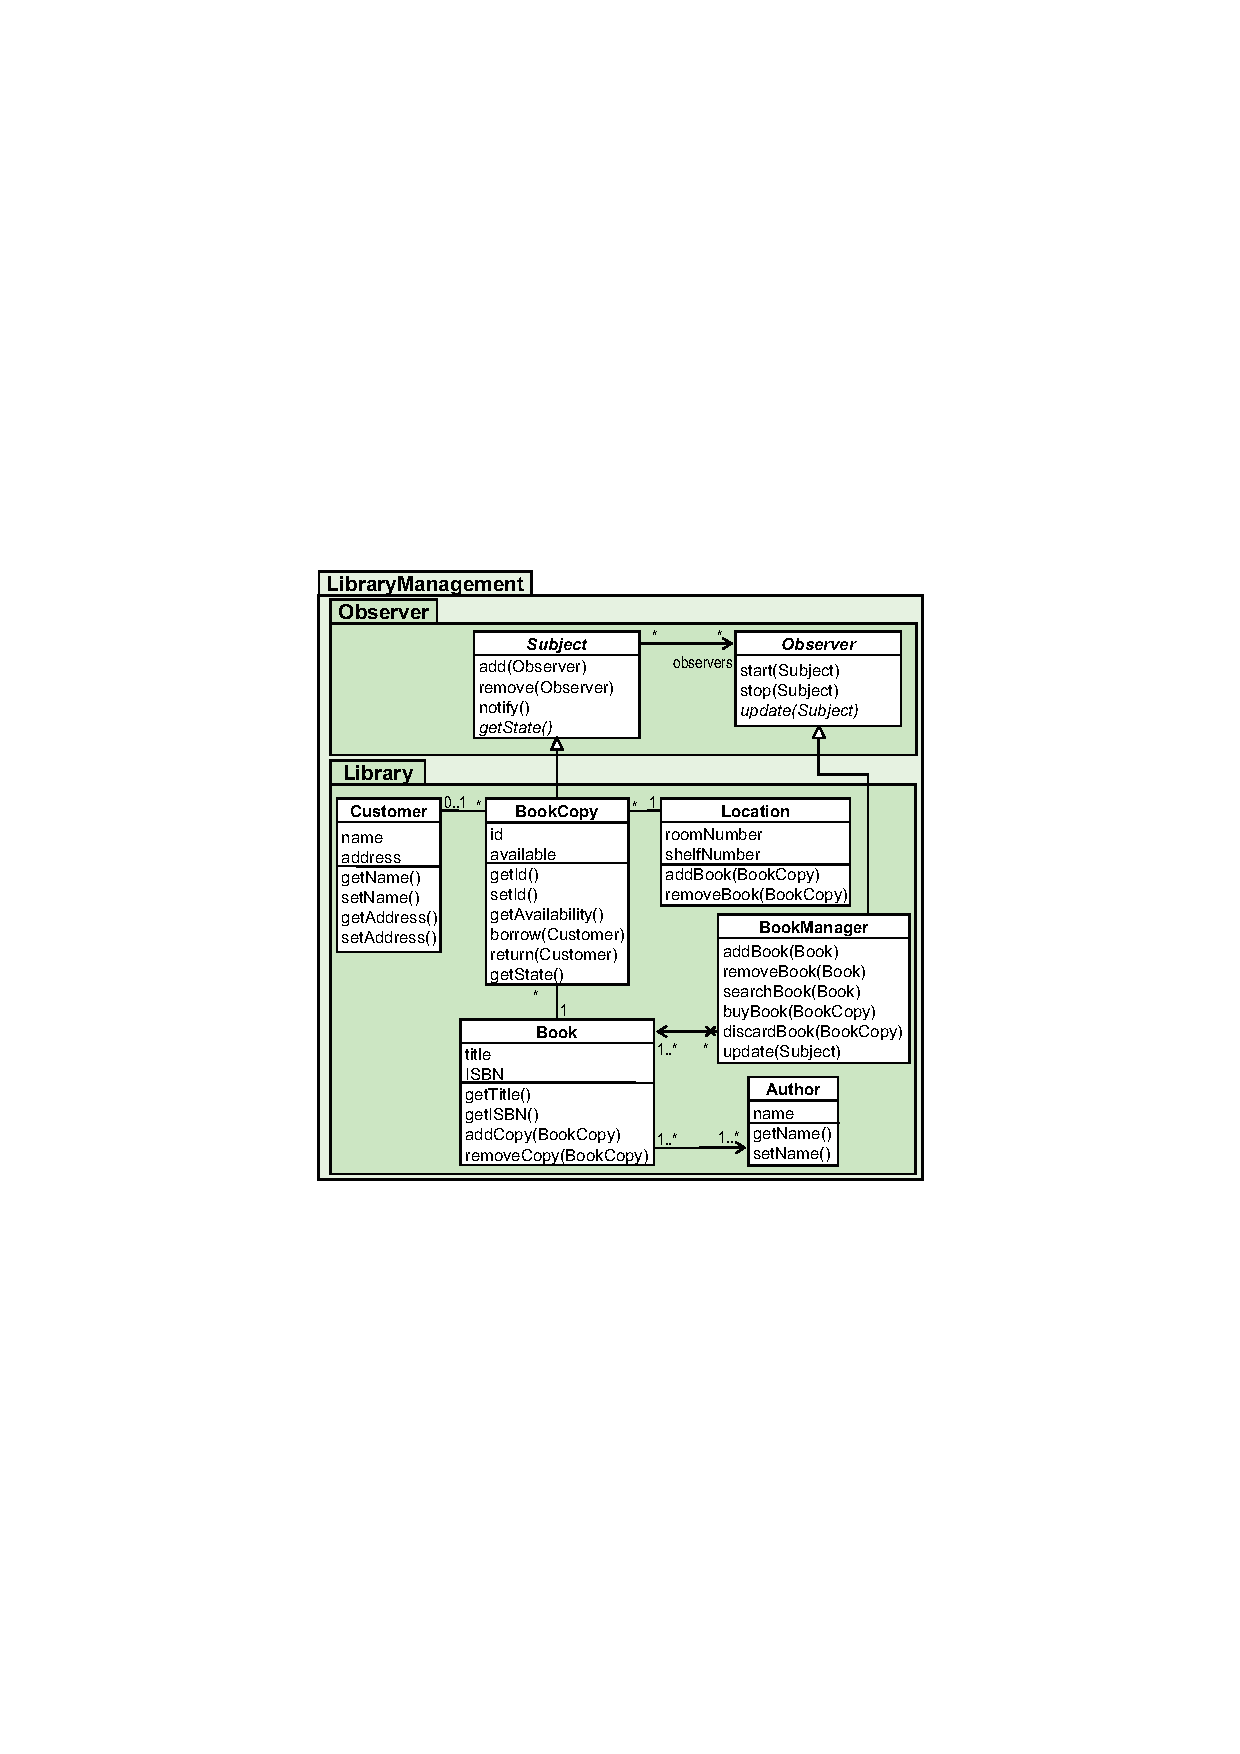
\includegraphics[width=0.7\textwidth]{figures/figure1}
	\caption{Sample figure}
	\label{fig:samplefigure_pdf}
\end{figure}


\section{Fonts}

When introducing important terms for the first time use \emph{emphasize}. For a consistent look and feel of proper names like {\cd} and {\uml{Observer}} pattern you may define macros in the main document \texttt{thesis.tex}.

\section{Code}

For short code fragments use the \textit{verbatim} environment.

\begin{verbatim}
//Start Program
System.out.println("Hello World!");
//End Program
\end{verbatim}

A much better alternative is the \textit{algorithm} environment (cf. Algorithm~\ref{alg:samplealgorithm}). This environment offers special formatting features for loops, operations and comments.

\begin{algorithm}[t]
\SetKwData{Left}{left}
\SetKwData{This}{this}
\SetKwData{Up}{up}
\SetKwFunction{Union}{Union}
\SetKwFunction{FindCompress}{FindCompress}
\SetKwInOut{Input}{input}
\SetKwInOut{Output}{output}

\Input{A bitmap $Im$ of size $w\times l$}
\Output{A partition of the bitmap}

\BlankLine

\emph{special treatment of the first line}\;
\For{$i\leftarrow 2$ \KwTo $l$}{
\emph{special treatment of the first element of line $i$}\;
\For{$j\leftarrow 2$ \KwTo $w$}{\label{forins}
\Left$\leftarrow$ \FindCompress{$Im[i,j-1]$}\;
\Up$\leftarrow$ \FindCompress{$Im[i-1,]$}\;
\This$\leftarrow$ \FindCompress{$Im[i,j]$}\;
\If(\tcp*[r]{O(\Left,\This)==1}){\Left compatible with \This}{\label{lt}
\lIf{\Left $<$ \This}{\Union{\Left,\This}}\;
\lElse{\Union{\This,\Left}\;}
}
\If(\tcp*[r]{O(\Up,\This)==1}){\Up compatible with \This}{\label{ut}
\lIf{\Up $<$ \This}{\Union{\Up,\This}}\;
\tcp{\This is put under \Up to keep tree as flat as possible}\label{cmt}
\lElse{\Union{\This,\Up}}\tcp*[r]{\This linked to \Up}\label{lelse}
}
}
\lForEach{element $e$ of the line $i$}{\FindCompress{p}}
}
\caption{Sample algorithm}\label{alg:samplealgorithm}
\end{algorithm}



%%%%%%%%%%%%%%%%%%%%%%%%%%%%%%%%%%%%%%%%%
\chapter{Bibliographic Issues}
\label{ch:bibliographic}
%%%%%%%%%%%%%%%%%%%%%%%%%%%%%%%%%%%%%%%%%

\section{Literature Search}

Information on online libraries and literature search, e.g., interesting magazines, journals, conferences, and organizations may be found at \url{http://www.big.tuwien.ac.at/teaching/info.html}.

\section{BibTeX}

BibTeX should be used for referencing.

The LaTeX source document of this pdf document provides you with different samples for references to journals~\cite{jour:B2BServices}, conference papers~\cite{proc:TheWebMLApproach}, books~\cite{book:umlatwork}, book chapters~\cite{incoll:ErhardKonrad1992}, electronic standards~\cite{man:BPEL}, dissertations~\cite{phdthesis:manuelWimmer}, masters' theses~\cite{mast:AUMLProfile}, and web sites~\cite{misc:BIGWebsite}. The respective BibTeX entries may be found in the file \texttt{references.bib}. For administration of the BibTeX references we recommend \url{http://www.citeulike.org} or JabRef for offline administration, respectively.


%%%%%%%%%%%%%%%%%%%%%%%%%%%%%%%%%%%%%%%%%
%%% BACKMATTER %%%%%%%%%%%%%%%%%%%%%%%%%%
%%%%%%%%%%%%%%%%%%%%%%%%%%%%%%%%%%%%%%%%%

\appendix

\bibliographystyle{plain}
\bibliography{references}

\end{document}
